\documentclass[12pt,a4paper]{article}
\usepackage[UTF8]{ctex}
\usepackage{amsmath}
\usepackage{graphicx}
\usepackage{booktabs}
\usepackage{geometry}
\usepackage{siunitx}
\usepackage{pgfplots}
\usepackage{ulem}
\usepackage{caption}
\pgfplotsset{compat=1.17}
\geometry{left=2.5cm,right=2.5cm,top=2.5cm,bottom=2.5cm}
\sisetup{per-mode=symbol}

\title{\Huge{\textbf{\uuline{实\ 验\ 报\ 告}}}}
\author{\uline{少年班学院} \quad 姓名: \uline{李大恕} \quad 学号: \uline{PB24000145}}
\date{\today}

\begin{document}
\maketitle

\section{实验题目}
闪烁体荧光衰减长度测量

\section{实验目的}
\begin{enumerate}
    \item 了解塑料闪烁计数器的一般结构、性能和应用。
    \item 初步了解一种测量长塑料闪烁体技术衰减长度的方法。
\end{enumerate}

\section{实验原理}
塑料闪烁体是在苯乙烯溶液中加入对联三苯（第一溶质）和 POPOP（第二溶质）聚合而成。带电粒子射入闪烁体后激发苯乙烯分子，其激发能传递给第一溶质，退激产生的光几乎全被第二溶质吸收，后者再次退激发出较长波长的可见光或紫光（3500$\sim$4800\,\AA），以便更好地匹配光电倍增管。

在塑料闪烁体中，光在透射过程中随距离按指数规律衰减。若强度为 $I_0$ 的光在闪烁体中传输距离 $x$\,(\unit{\centi\meter})，其光强度 $I$ 满足：
\begin{equation}
    I = I_0 \mathrm{e}^{-\mu x},
\end{equation}
即
\begin{equation}
    \ln I = -\mu x + \ln I_0,
\end{equation}
其中 $\mu$ 为光在闪烁体和光导中的有效吸收系数。通常定义衰减长度 $\lambda = 1/\mu$，表示光强衰减到 $1/\mathrm{e}$ 时的传输距离。由于未经波长过滤，此处测得的为有效技术衰减长度。

光子经光导衰减后被光阴极收集，经电子倍增在阳极产生电压脉冲 $V$，由线性关系 $V = kI$ (其中 $k$ 为常数) 可得：
\begin{equation}
    V = V_0 \mathrm{e}^{-\mu x},
\end{equation}
取对数有
\begin{equation}
    \ln V = -\mu x + \ln V_0.
    \label{eq:lnV}
\end{equation}
在此原理下，通过固定扣除本底后的纯计数率以标定某一等效光强，并测量此时的甄别阈值 $V$ 随射线源与光阴极距离 $x$ 的关系，再根据最小二乘法对 $\ln V$ 与 $x$ 作线性拟合即可得衰减参量 $\mu$ 与有效技术衰减长度。

\section{实验装置和步骤}
实验仪器包括：单道闪烁能谱仪一套、长塑料闪烁体一块（带探头）、$^{90}\mathrm{Sr}\text{--}^{90}\mathrm{Yb}$ $\beta$ 放射源一个、示波器一台。

具体步骤如下：
\begin{enumerate}
    \item 探头检查：将整个闪烁计数器用黑布包住，接通电源并缓慢加高压。开启定标器，逐步掀开黑布以检查漏光。若本底计数增加说明漏光，需重新密封，直至彻底掀开黑布后本底计数无明显增加。
    \item 脉冲波形观察：用示波器观察光电倍增管输出信号脉冲的前沿特性。
    \item 测量有效技术衰减长度：调节放射源位置与单道分析器阈值 $V_T$，使多次测得纯计数 $N - N_b$ 保持在 $5000\pm200$ 左右，记录对应距离 $x$ (\unit{\centi\meter}) 和相应的甄别阈值 $V_T$ (\unit{\volt})。
\end{enumerate}

\section{数据处理与结果}
实验所测原始数据如下表所示。纯计数 $N - N_b$ 为每次测量计数 $N$ 与本底计数 $N_b$ 之差，要求相对统计误差小于 1.5\%。针对每一阈值 $V_T$ 进行了三次重复计数。

\begin{table}[htbp]
\centering
\caption{不同位置 $x$ 及甄别阈值 $V_T$ 下的数据记录}
\begin{tabular}{ccccc}
\toprule
$x$ / \unit{\centi\meter} & $V_T$ / \unit{\volt} & $N$ & $N_b$ & $N-N_b$ \\
\midrule
20 & 4.30 & 6188, 6098, 6002 & 1051, 991, 983 & 5137, 5107, 5019 \\
30 & 3.70 & 6317, 6275, 6439 & 1347, 1359, 1360 & 4970, 4916, 5079 \\
40 & 3.30 & 6788, 6680, 6739 & 1632, 1603, 1562 & 5156, 5077, 5177 \\
50 & 3.00 & 6932, 6904, 6848 & 1886, 1832, 1829 & 5046, 5072, 5019 \\
60 & 2.70 & 7237, 7171, 7203 & 2274, 2180, 2176 & 4963, 4991, 5027 \\
70 & 2.45 & 7373, 7364, 7308 & 2350, 2273, 2328 & 5023, 5091, 4980 \\
80 & 2.20 & 7678, 7671, 7785 & 2712, 2678, 2750 & 4966, 4993, 5035 \\
90 & 2.05 & 7844, 7878, 7858 & 2873, 2834, 2960 & 4971, 5044, 4898 \\
100 & 1.90 & 8015, 7940, 8020 & 2991, 2951, 3034 & 5024, 4989, 4986 \\
110 & 1.78 & 8077, 8083, 8212 & 3197, 3167, 3158 & 4880, 4916, 5054 \\
\bottomrule
\end{tabular}
\end{table}

为了求得衰减长度，对每一组距离 $x$ 与甄别阈值 $V_T$ 进行坐标变换，计算 $\ln V_T$。

\begin{figure}[htbp]
\centering
\begin{tikzpicture}
\begin{axis}[
    width=0.88\textwidth,
    height=0.55\textwidth,
    xlabel={距离 $x$ (\unit{\centi\meter})},
    ylabel={$\ln V_T$},
    xmin=10, xmax=120,
    ymin=0.4, ymax=1.6,
    grid=both,
    legend pos=north east
]
\addplot[blue, mark=*, only marks] coordinates {
    (20, 1.4586)
    (30, 1.3083)
    (40, 1.1939)
    (50, 1.0986)
    (60, 0.9933)
    (70, 0.8961)
    (80, 0.7885)
    (90, 0.7178)
    (100, 0.6419)
    (110, 0.5766)
};
\addplot[red, thick, domain=10:120] {-0.00976*x + 1.602};
\legend{实验数据点, 线性拟合}
\end{axis}
\end{tikzpicture}
\caption{$\ln V_T$ 随 $x$ 变化的线性关系拟合}
\end{figure}

依公式~\eqref{eq:lnV}，将 $x$ 和对应的 $\ln V_T$ 进行最小二乘法线性回归拟合得到斜率 $-\mu$。具体计算为：
\begin{align*}
    \mu &= -\frac{\sum (x_i - \bar{x})(\ln V_i - \overline{\ln V})}{\sum (x_i - \bar{x})^2} \approx 0.009704 \ \unit{\centi\meter^{-1}},
\end{align*}
其对应的有效技术衰减长度定为 $\lambda = 1/\mu$。可得：
\begin{equation}
    \lambda \approx 103.0 \ \unit{\centi\meter}.
\end{equation}

通过测量，我们得到了塑料闪烁体的有效衰减特性。

\newpage

\appendix
\section{原始数据记录}
下面为包含本组实验原始手动数据记录和教师电子手写签名的扫描件。
\begin{figure}[htbp]
    \centering
    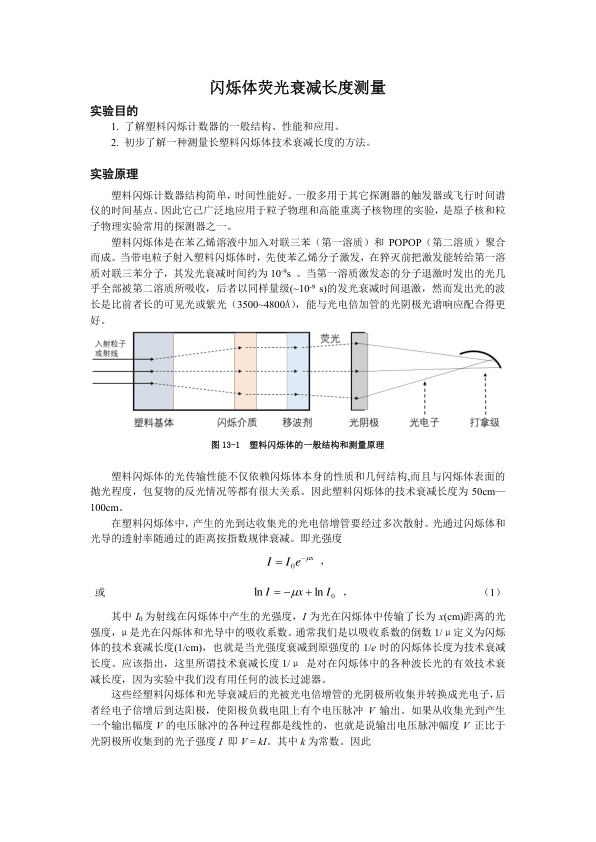
\includegraphics[width=0.7\textwidth]{assets_data/page1_render.png}
    \caption{附带教师电子手写签名的原始扫描数据}
\end{figure}

\end{document}